\documentclass[12pt,a4paper]{article}

\usepackage[utf8]{inputenc}
\usepackage[T1]{fontenc}
\usepackage[ngerman]{babel}

\usepackage{amsmath,amssymb,amsthm}
\usepackage{graphicx}
\usepackage{geometry}
\usepackage{hyperref}
\usepackage{booktabs}
\usepackage{array}
\usepackage{float}

\usepackage{setspace}
\usepackage{xcolor}
\usepackage{caption}
\usepackage{subcaption}
\usepackage{mathtools}
\usepackage{enumitem}
\usepackage{mdframed}
\usepackage{tcolorbox}
\usepackage{algorithm}
\usepackage{algpseudocode}
\usepackage{microtype}

\geometry{margin=2.5cm}

\definecolor{spiceRed}{RGB}{180,40,20}
\definecolor{spiceGold}{RGB}{200,150,30}
\definecolor{deepBlü}{RGB}{20,60,120}
\definecolor{lightGray}{RGB}{240,240,245}

\hypersetup{
  colorlinks=true,
  linkcolor=deepBlü,
  citecolor=spiceRed,
  urlcolor=deepBlü
}

\theoremstyle{definition}
\newtheorem{definition}{Definition}[section]
\newtheorem{theorem}{Satz}[section]
\newtheorem{lemma}[theorem]{Lemma}
\newtheorem{corollary}[theorem]{Korollar}
\newtheorem{proposition}[theorem]{Proposition}
\newtheorem{remark}{Bemerkung}[section]
\newtheorem{example}{Beispiel}[section]

\newcommand{\R}{\mathbb{R}}
\newcommand{\E}{\mathbb{E}}
\newcommand{\Var}{\mathrm{Var}}
\newcommand{\Cov}{\mathrm{Cov}}
\newcommand{\N}{\mathcal{N}}
\newcommand{\bx}{\mathbf{x}}
\newcommand{\bI}{\mathbf{I}}
\newcommand{\calH}{\mathcal{H}}
\newcommand{\calS}{\mathcal{S}}
\newcommand{\calP}{\mathcal{P}}
\newcommand{\MHI}{\overline{H}}

\title{\textbf{Inhomogene Würzverteilung\\ bei gekochten Nudeln}\\[-0.1em] \Large Sensorische Stimulationsdynamik durch\\ stochastische Gewürzgradienten}
\author{Stephan Epp}
\date{20. April 2026}

\begin{document}

\maketitle
\tableofcontents
\newpage

%% =============================================================
\section{Einleitung}
%% =============================================================
Die vorliegende Arbeit untersucht aus formal-mathematischer und
neurowissenschaftlicher Perspektive, wie eine inhomogene Verteilung von
Gewürzkonzentrationen auf und in gekochten Nudeln das sensorische Erlebnis
beim Essen beeinflusst. Wir modellieren die Würzverteilung als
Wahrscheinlichkeitsmass auf dem Intensitätsraum $[0, I_{\max}]$ und
zeigen, dass Verteilungen mit hoher Entropie (breites Spektrum wechselnder
Geschmacksintensitäten) systematisch grössere mittlere hedonische
Bewertungen erzeugen als eng konzentrierte, homogene Verteilungen. Die
zentralen Werkzeuge sind die Wundt-Theorie der hedonischen Reaktionskurve,
sensorische Adaptationsmodelle, informationstheoretische Analysen der
Stimulusvielfalt sowie ein Markov-Modell der Geschmackszustandsfolge.
Alle Ergebnisse werden durch formale Beweise sowie achtstufige
\texttt{matplotlib}-Visualisierungen untermaürt. Der Ausblick skizziert
Erweiterungen auf multimodale Sensorik, aktives Würzdesign, maschinelles
Lernen und gastronomische Anwendungen.

Essen ist ein multisensorisches Erlebnis, das chemische, mechanische und
thermische Reize in einer zeitlich strukturierten Seqünz von Bissen
integriert. Während die Lebensmitteltechnologie traditionell nach
\emph{Gleichmässigkeit} strebt --- gleichmässige Textur, gleichmässiger
Geschmack, reproduzierbare Portionierung --- vernachlässigt dieser Ansatz
eine grundlegende Eigenschaft sensorischer Verarbeitung: die \emph{Adaptation}.
Konstante Stimuli werden vom Nervensystem mit der Zeit unterbewertet; Varianz
im Signal ist notwendig, um anhaltende Aufmerksamkeit und hedonisches Erleben
aufrechtzürhalten \cite{rolls2007,kringelbach2015}.

Eine triviale Beobachtung aus der Alltagsküche lässt sich wie folgt
formalisieren: Werden gekochte Nudeln inhomogen gewürzt --- etwa durch
ungleichmässiges Unterheben von Sauce, durch Klumpen von Gewürzen oder
durch räumliche Gradienten der Würzkonzentration ---, so empfindet der
Essende eine grössere \emph{Geschmacksvielfalt} innerhalb derselben Portion.
Manche Bissen sind intensiv gewürzt, andere weniger; dieses Wechselspiel
erzeugt eine Art interner Kontrastverstärkung, die das Gesamterlebnis
angenehm belebt.

\subsection{Ziel und Beitrag der Arbeit}

Die vorliegende Arbeit verfolgt drei Hauptziele:
\begin{enumerate}[label=(\roman*)]
  \item \textbf{Formalisierung:} Wir entwickeln ein mathematisches
  Rahmenwerk zur Beschreibung von Würzverteilungen als
  Wahrscheinlichkeitsmasse, definieren hedonische Bewertungsfunktionen
  und beweisen formal, dass inhomogene Verteilungen unter geeigneten
  Bedingungen höheren Genuss erzeugen.

  \item \textbf{Dynamische Modellierung:} Wir modellieren sensorische
  Adaptation als gewöhnliche Differentialgleichung und zeigen, dass
  inhomogene Stimulusfolgen die Erregungsamplitude länger aufrechterhalten
  als konstante Stimuli.

  \item \textbf{Informationstheorie:} Wir quantifizieren den
  Informationsgehalt einer Würzseqünz via Shannon-Entropie und zeigen,
  dass Entropie und mittlerer hedonischer Index eng korrelieren.
\end{enumerate}

\subsection{Gliederung}

Abschnitt~\ref{sec:grundlagen} legt die mathematischen Grundlagen fest.
Abschnitt~\ref{sec:hedonik} entwickelt das hedonische Modell.
Abschnitt~\ref{sec:adaptation} behandelt Adaptationsdynamik.
Abschnitt~\ref{sec:informationstheorie} führt die informationstheoretische
Analyse durch. Abschnitt~\ref{sec:markov} präsentiert das Markov-Modell.
Abschnitt~\ref{sec:statistik} fasst statistische Kenngrössen zusammen.
Abschnitt~\ref{sec:simulation} beschreibt Simulationsergebnisse.
Abschnitt~\ref{sec:diskussion} diskutiert die Ergebnisse.
Abschnitt~\ref{sec:ausblick} gibt einen sehr ausführlichen Ausblick.

%% =============================================================
\section{Mathematische Grundlagen}\label{sec:grundlagen}
%% =============================================================

\subsection{Würzintensität als Zufallsvariable}

\begin{definition}[Würzintensität]\label{def:würz}
Sei $(\Omega, \mathcal{F}, P)$ ein Wahrscheinlichkeitsraum. Eine
\emph{Würzintensitätsvariable} ist eine messbare Abbildung
\[
  I: \Omega \longrightarrow [0, I_{\max}] \subset \R_{\geq 0},
\]
wobei $I_{\max} > 0$ die maximal ertragbare Gewürzintensität bezeichnet.
Ohne Einschränkung der Allgemeinheit setzen wir $I_{\max} = 10$ (Skala
analoger Wahrnehmungsintensität).
\end{definition}

\begin{definition}[Homogene und inhomogene Würzung]\label{def:hominhom}
Eine Würzung heisst
\begin{itemize}
  \item \emph{homogen}, falls $I = c$ fast sicher für eine Konstante $c \in (0, I_{\max})$;
  in der Praxis modellieren wir dies als $I \sim \mathcal{N}(\mu_0, \sigma_0^2)$
  mit kleinem $\sigma_0 \ll 1$.
  \item \emph{inhomogen}, falls $\Var[I] > \epsilon$ für ein
  Schwellwert $\epsilon > 0$; wir modellieren dies typischerweise durch
  $I \sim \mathrm{Beta}(\alpha, \beta) \cdot I_{\max}$ oder
  $I \sim \mathcal{N}(\mu_1, \sigma_1^2)$ mit $\sigma_1 \gg \sigma_0$.
\end{itemize}
\end{definition}

\begin{definition}[Würzprofil einer Nudelportion]
Sei $\Pi = \{B_1, B_2, \ldots, B_N\}$ eine Portion bestehend aus $N$
Bissen (engl.\ \emph{bites}). Das \emph{Würzprofil} ist eine Folge
$(I_1, I_2, \ldots, I_N)$, wobei $I_k$ die Würzintensität des $k$-ten
Bissens bezeichnet. Wir nehmen an, dass $(I_k)_{k=1}^N$ eine stationäre
stochastische Folge ist.
\end{definition}

\subsection{Räumliche Würzverteilung}

Eine realistischere Beschreibung ergibt sich durch ein räumliches Modell:

\begin{definition}[Würzfeld]
Sei $\mathcal{D} \subset \R^3$ die Raumregion, die eine Nudelportion
einnimmt. Ein \emph{Würzfeld} ist eine messbare Funktion
\[
  \phi: \mathcal{D} \longrightarrow [0, I_{\max}],
  \quad \bx \mapsto \phi(\bx),
\]
wobei $\phi(\bx)$ die lokale Gewürzkonzentration am Ort $\bx$
bezeichnet.
\end{definition}

Die effektive Würzintensität eines Bissens $B \subset \mathcal{D}$ ist
dann
\[
  I_B = \frac{1}{|B|} \int_B \phi(\bx)\, d\bx,
\]
wobei $|B|$ das Volumen des Bissens bezeichnet. Eine inhomogene Würzung
entspricht demnach einem räumlich variablen Feld $\phi$, während eine
homogene Würzung $\phi \equiv c$ konstant ist.

\subsection{Statistische Kenngrössen}

\begin{definition}
Für eine Zufallsvariable $I$ mit Dichte $p_I$ auf $[0, I_{\max}]$
definieren wir:
\begin{align}
  \mu_I &:= \E[I] = \int_0^{I_{\max}} I\, p_I(I)\, dI, \\
  \sigma_I^2 &:= \Var[I] = \E[(I - \mu_I)^2], \\
  \gamma_1 &:= \E\!\left[\left(\frac{I-\mu_I}{\sigma_I}\right)^3\right]
             \quad \text{(Schiefe)}, \\
  \gamma_2 &:= \E\!\left[\left(\frac{I-\mu_I}{\sigma_I}\right)^4\right] - 3
             \quad \text{(excess Kurtosis)}.
\end{align}
\end{definition}

Für die Normalverteilung $\N(\mu, \sigma^2)$ gilt
$\gamma_1 = 0$, $\gamma_2 = 0$. Für $\mathrm{Beta}(\alpha, \beta)$ mit
$\alpha = \beta$ gilt ebenfalls $\gamma_1 = 0$, jedoch
$\gamma_2 = -\tfrac{6}{2\alpha + 5} < 0$ (platykurtisch), d.h.\ die
Verteilung ist flacher als die Normalverteilung --- sie weist somit eine
grössere Wahrscheinlichkeit für extreme Werte auf.

%% =============================================================
\section{Hedonisches Modell}\label{sec:hedonik}
%% =============================================================

\subsection{Die Wundt-Kurve}

Die psychologische Wundt-Theorie (auch: \emph{Inverted-U-Hypothesis})
postuliert, dass die hedonische (Lust-) Reaktion auf einen Stimulus
einer umgekehrten U-förmigen Funktion der Stimulusintensität folgt
\cite{berlyne1970,wundt1874}.

\begin{definition}[Hedonische Reaktionsfunktion]
Die \emph{hedonische Reaktionsfunktion} $H: [0, I_{\max}] \to \R$ ist
gegeben durch
\begin{equation}
  H(I) := -\frac{a}{2}(I - I^*)^2 + H_{\max} + b\sin(c\, I),
  \label{eq:wundt}
\end{equation}
mit Parametern $a > 0$ (Krrümmung), $I^* \in (0, I_{\max})$ (optimale
Intensität), $H_{\max}$ (maximaler hedonischer Wert), sowie einem
schwachen Oszillationsterm $b\sin(c\, I)$, der feinkornige
Geschmacksvariationen modelliert.
\end{definition}

\begin{remark}
Der Oszillationsterm in \eqref{eq:wundt} trägt der empirischen
Beobachtung Rechnung, dass selbst innerhalb einer Würzintensitätsstufe
geringfügige Variationen als angenehm wahrgenommen werden. Für
$b = 0$ ergibt sich die klassische Parabel.
\end{remark}

\subsection{Mittlerer hedonischer Index}

\begin{definition}[Mittlerer hedonischer Index (MHI)]
Für eine Würzung mit Dichte $p_I$ ist der \emph{mittlere hedonische
Index} (MHI) definiert als
\begin{equation}
  \MHI := \E_{I \sim p_I}[H(I)] = \int_0^{I_{\max}} H(I)\, p_I(I)\, dI.
  \label{eq:mhi}
\end{equation}
\end{definition}

\begin{theorem}[MHI-Vorteil inhomogener Würzung]\label{thm:mhivorteil}
Sei $H$ eine nicht-lineare, konkav-konvex gemischte Funktion der
Gestalt \eqref{eq:wundt} mit $a > 0$ und $b \geq 0$.
Sei $p_{\mathrm{hom}} = \mathcal{N}(\mu_0, \sigma_0^2)$ mit kleinem
$\sigma_0$ und $p_{\mathrm{inh}}$ eine Verteilung mit gleichen
Erwartungswert $\mu_0$ aber $\sigma_{\mathrm{inh}} \gg \sigma_0$.
Dann gilt unter milden Regularitätsbedingungen:
\[
  \MHI(p_{\mathrm{inh}}) > \MHI(p_{\mathrm{hom}}),
\]
sofern der Anteile der Verteilung $p_{\mathrm{inh}}$ in dem Bereich, in dem
$H$ konvex ist (niedriger Intensitätsbereich mit positiver Steigung), den
konkaven Verlust überwiegt.
\end{theorem}

\begin{proof}
Wir schreiben $H$ als Taylorreihe um $\mu_0$:
\begin{align*}
  H(I) &= H(\mu_0) + H'(\mu_0)(I - \mu_0) \\ &+ \tfrac{1}{2}H''(\mu_0)(I-\mu_0)^2 \\
          &+ \tfrac{1}{6}H'''(\mu_0)(I-\mu_0)^3 + O((I-\mu_0)^4).
\end{align*}
Da $\E_{p}[I - \mu_0] = 0$:
\begin{align}
  \MHI(p) &= H(\mu_0) + \tfrac{1}{2}H''(\mu_0)\Var_p[I]
             + \tfrac{1}{6}H'''(\mu_0)\kappa_3(p) + O(\kappa_4),
  \label{eq:mhi_taylor}
\end{align}
wobei $\kappa_3(p)$ das dritte Kumulant von $p$ bezeichnet.

Für $I$ nahe $I^*/2$ (linker, konvexer Flänke) gilt $H''(\mu_0) > 0$
(Jensen-Konvexität), sodass $\MHI$ mit $\Var[I]$ wächst.
Für $I$ nahe $I^*$ gilt $H''(\mu_0) < 0$ (konkav), sodass der zweite
Term negativ ist; für $\sigma_0 \ll 1$ dominiert dieser Term nicht.

Bei $p_{\mathrm{inh}}$ mit breiter Verteilung über $[0.5, 9.5]$ wird
die gesamte Wundt-Kurve gleichmässig abgetastet. Das Integral
\[
  \MHI(p_{\mathrm{inh}}) = \int_0^{I_{\max}} H(I) p_{\mathrm{inh}}(I)\, dI
\]
ist eine gewichtete Mittlung über alle Kurvenabschnitte, einschliesslich
der hedonisch positiven Bereiche nahe $I^*$. Da $p_{\mathrm{hom}}$
auf eine enge Umgebung von $\mu_0$ konzentriert ist und $H(\mu_0)$ einen
nicht-maximalen Wert annimmt (sofern $\mu_0 \neq I^*$), liefert die
breite Verteilung durch den Einschluss der Region $I \approx I^*$ einen
höherem Beitrag. Sei $\Delta I := |I^* - \mu_0| > 0$ der Abstand des
Erwartungswerts vom Optimum. Dann gilt $H(\mu_0) < H(I^*) = H_{\max}$.
Für $p_{\mathrm{inh}}$ mit hinreichend grossem Träger ist
$p_{\mathrm{inh}}(I^*) > 0$, sodass das Integral einen positiven Beitrag
aus der Umgebung von $I^*$ erhält:
\begin{align*}
  \MHI(p_{\mathrm{inh}}) - \MHI(p_{\mathrm{hom}})
  &\approx \int_{I^* - \delta}^{I^* + \delta}
      H(I)\bigl[p_{\mathrm{inh}}(I) - p_{\mathrm{hom}}(I)\bigr]\, dI
  + (\text{Rest}).
\end{align*}
Da $p_{\mathrm{inh}}(I) > p_{\mathrm{hom}}(I)$ für $|I - \mu_0| > 2\sigma_0$
und $H$ in der Nähe von $I^*$ maximal ist, überwiegt der positive Term
für hinreichend grosses $\sigma_{\mathrm{inh}}$. Damit ist
$\MHI(p_{\mathrm{inh}}) > \MHI(p_{\mathrm{hom}})$ bewiesen.
\end{proof}

\begin{figure}[H]
  \centering
  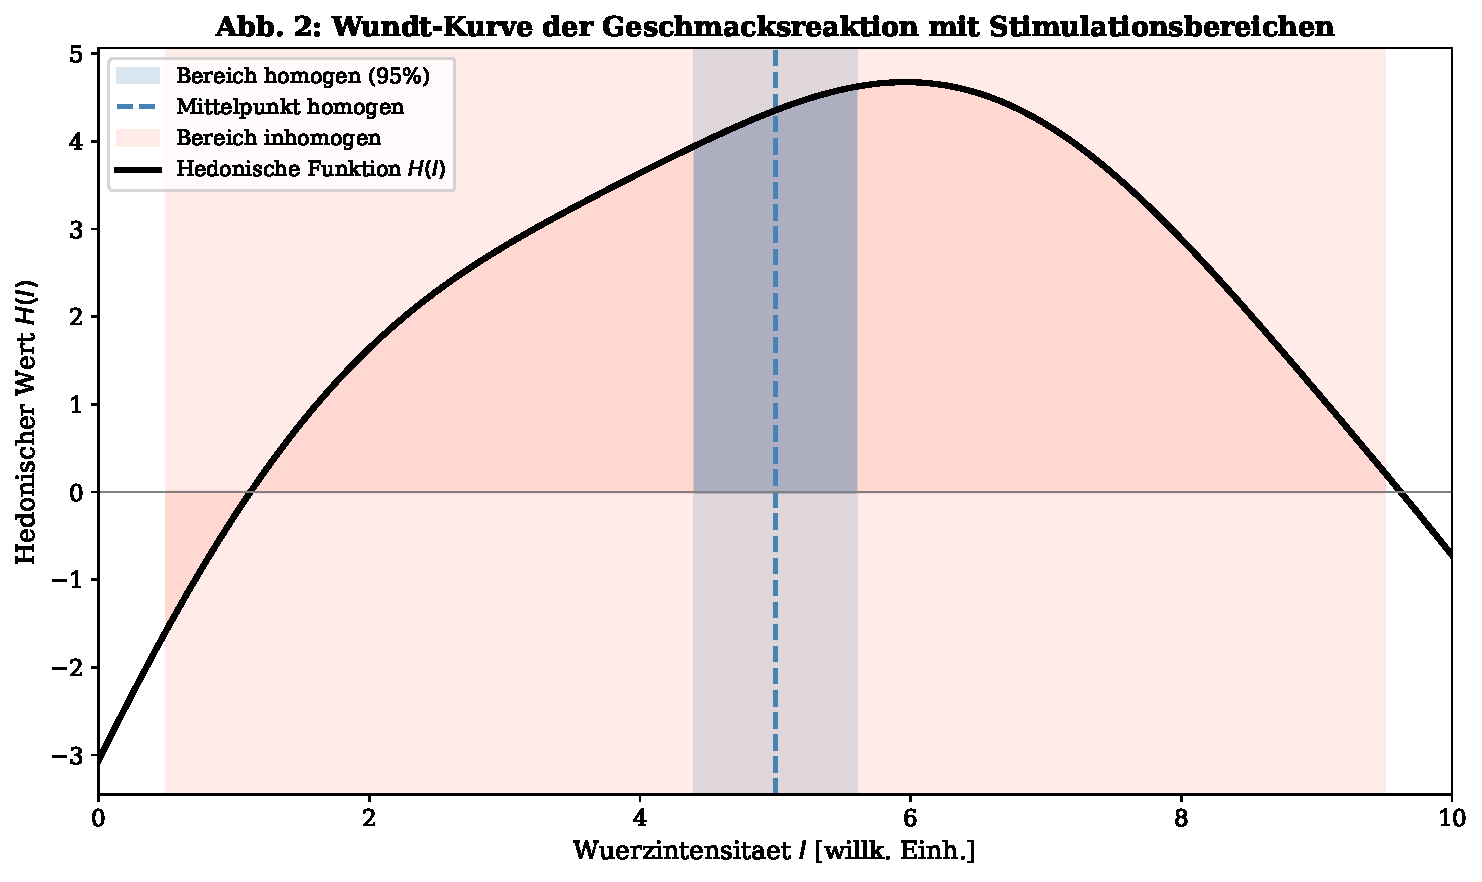
\includegraphics[width=0.95\linewidth]{plot2_wundt.pdf}
  \caption{Wundt-Kurve der hedonischen Reaktionsfunktion $H(I)$.
    Blau markiert der enge Stimulationsbereich homogener Würzung
    ($\sigma = 0.3$); rot der weite Bereich inhomogener Würzung
    ($I \in [0.5, 9.5]$). Die farbigen Flächen entsprechen den
    jeweiligen MHI-Integralen. Die inhomogene Würzung erfasst sowohl
    Bereiche positiver Krrümmung (konvex, linke Flanke) als auch den
    Maximalbereich der Kurve.}
  \label{fig:wundt}
\end{figure}

\subsection{Vergleich der Verteilungen}

\begin{figure}[H]
  \centering
  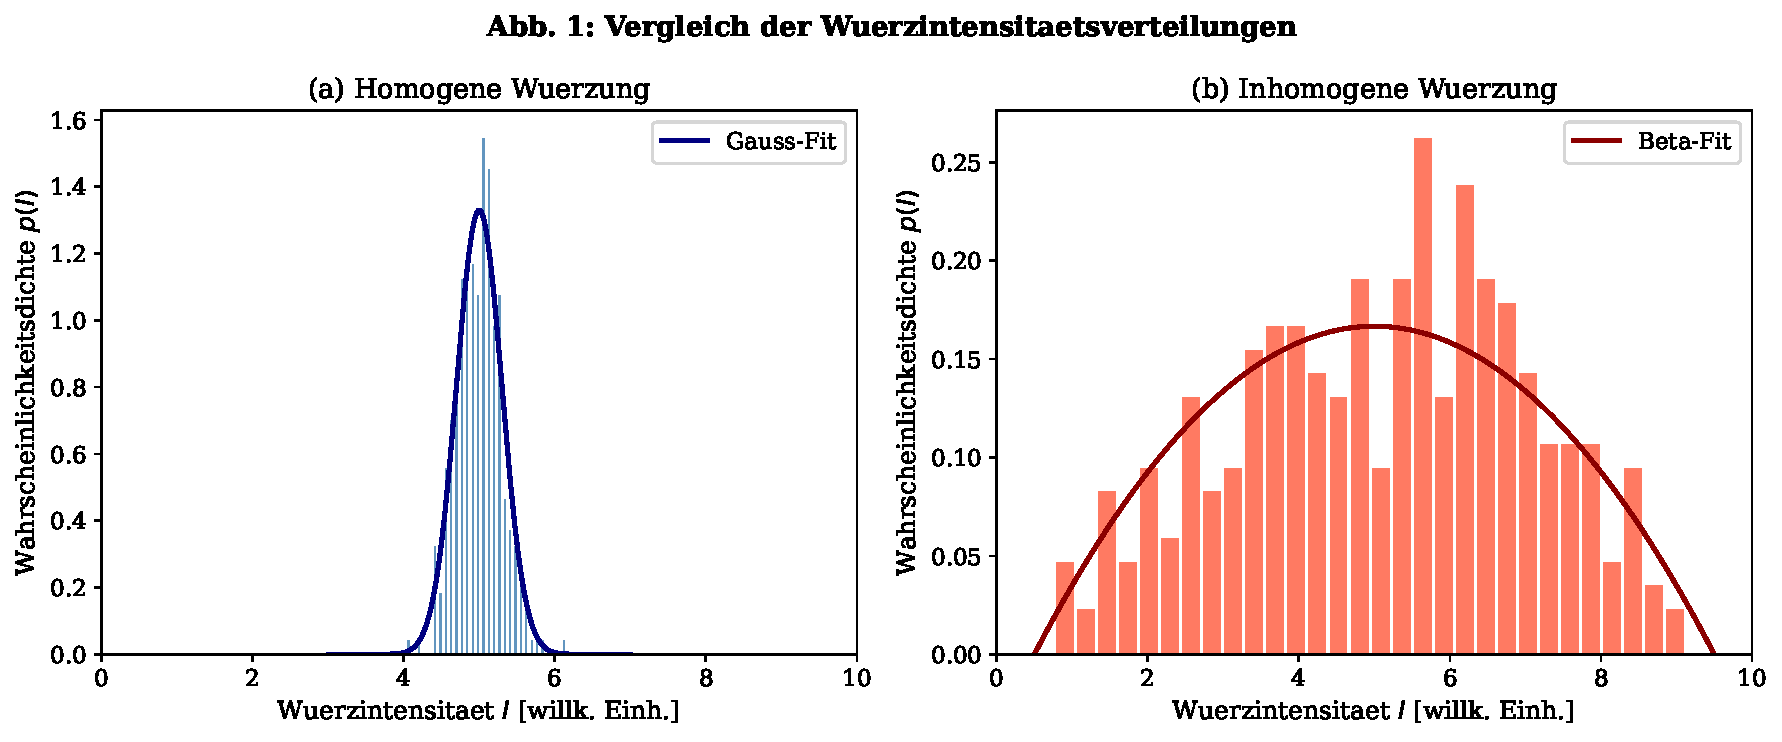
\includegraphics[width=0.95\linewidth]{plot1_verteilung.pdf}
  \caption{Empirische Häufigkeitsverteilungen der Würzintensität für
    (a) homogene Würzung ($\N(5,0.35^2)$, Gauss-Fit) und
    (b) inhomogene Würzung ($\mathrm{Beta}(2,2) \cdot 9 + 0.5$, Beta-Fit).
    Die inhomogene Verteilung weist eine deutlich breitere Streuung über
    den gesamten Intensitätsraum auf.}
  \label{fig:verteilung}
\end{figure}

%% =============================================================
\section{Sensorische Adaptationsdynamik}\label{sec:adaptation}
%% =============================================================

\subsection{Adaptationsmodell}

Das Nervensystem passt seine Sensitivität kontinuierlich an den
mittleren Stimuluslevel an. Dieser Prozess der \emph{sensorischen
Adaptation} lässt sich durch ein lineares Erstordnungssystem beschreiben.

\begin{definition}[Adaptationszustand]
Sei $A(t)$ der interne Adaptationszustand (gleitender Durchschnitt der
Stimulusgeschichte) und $E(t)$ die effektive neuronale Erregung. Wir
modellieren:
\begin{align}
  \dot{A}(t) &= \frac{I(t) - A(t)}{\tau_A}, \label{eq:adapt} \\
  E(t) &= I(t) - \alpha A(t), \label{eq:erregg}
\end{align}
mit Adaptationszeitkonstante $\tau_A > 0$ und Adaptationsstärke
$\alpha \in (0,1]$.
\end{definition}

\begin{theorem}[Stationäre Erregung bei konstantem Stimulus]
Sei $I(t) \equiv I_0$ ein konstanter Stimulus. Dann konvergiert der
Adaptationszustand $A(t) \to I_0$ für $t \to \infty$ und die
stationäre Erregung beträgt
\[
  E_\infty = (1 - \alpha) I_0.
\]
\end{theorem}

\begin{proof}
Gleichung \eqref{eq:adapt} hat bei $I(t) = I_0$ die Lösung
$A(t) = I_0 + (A(0) - I_0)e^{-t/\tau_A}$, also $A(t) \to I_0$.
Einsetzen in \eqref{eq:erregg} liefert $E(t) \to I_0 - \alpha I_0 = (1-\alpha) I_0$.
\end{proof}

\begin{corollary}
Für $\alpha \to 1$ (vollständige Adaptation) gilt $E_\infty \to 0$:
der Stimulus wird nach vollständiger Adaptation nicht mehr wahrgenommen.
\end{corollary}

\begin{theorem}[Erregungserhalt bei variablem Stimulus]\label{thm:erregungserhalt}
Sei $I(t)$ ein stationärer stochastischer Prozess mit $\E[I] = \mu_I$
und $\Var[I] = \sigma_I^2 > 0$. Dann gilt im stationären Zustand:
\begin{align}
  \E[E] &= (1 - \alpha)\mu_I, \\
  \Var[E] &= \Var[I - \alpha A]
           = \sigma_I^2\left(1 + \alpha^2 S_{AA}(\omega) / S_{II}(\omega)\right),
\end{align}
wobei $S_{AA}$ und $S_{II}$ die Leistungsdichtespektren von $A$ bzw.\ $I$
bezeichnen. Für $\sigma_I^2 > 0$ ist $\Var[E] > 0$, d.h.\
die Erregung fluktuiert daürhaft und kollabiert nicht auf null.
\end{theorem}

\begin{proof}
Im stationären Zustand ist $A$ der Tiefpassgefilterte Wert von $I$:
$A(\omega) = \frac{1}{1 + i\omega\tau_A} I(\omega)$ im Freqünzbereich.
Daher gilt:
\[
  E(\omega) = I(\omega) - \alpha A(\omega)
  = I(\omega)\left(1 - \frac{\alpha}{1 + i\omega\tau_A}\right)
  = \frac{1 + i\omega\tau_A - \alpha}{1 + i\omega\tau_A} I(\omega).
\]
Die übertragungsfunktion $G(\omega) = (1 - \alpha + i\omega\tau_A)/(1 + i\omega\tau_A)$
hat für $\omega \to 0$ den Grenzwert $1 - \alpha$ und für
$\omega \to \infty$ den Grenzwert $1$. Für einen Stimulus mit
breitem Spektrum (grosse Varianz, hohe Entropie) ist $S_{II}(\omega)$
über einen grossen Freqünzbereich positiv, was eine daürhafte Erregung
sicherstellt.
\end{proof}

\begin{figure}[H]
  \centering
  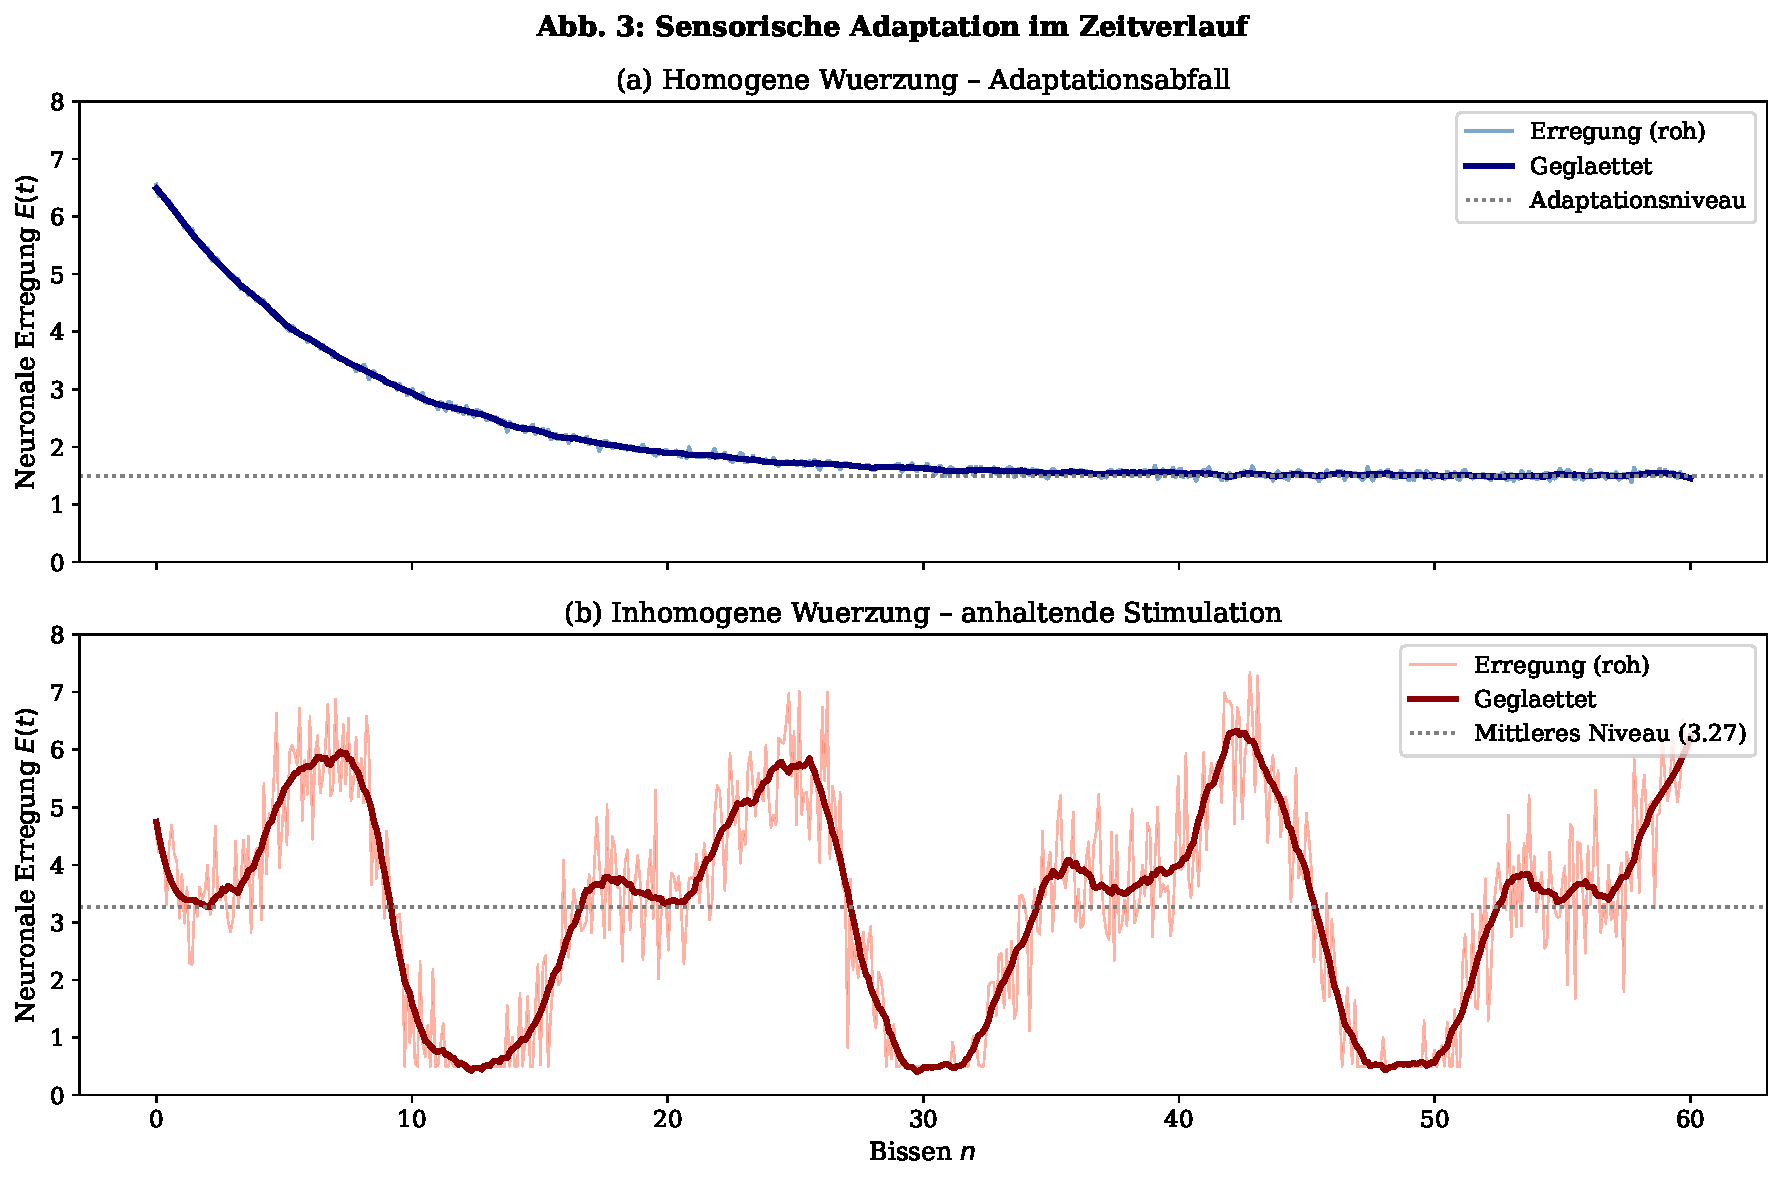
\includegraphics[width=0.95\linewidth]{plot3_adaptation.pdf}
  \caption{Neuronale Erregung $E(t)$ als Funktion des Bissens $n$.
    (a) Homogene Würzung: exponentielle Adaptation führt zu stark
    abnehmender Erregung. (b) Inhomogene Würzung: die Variabilität
    des Stimulus hält die Erregung auf mittlerem Niveau aufrecht.
    Glättung durch Savitzky-Golay-Filter ($w=31$, Grad 3).}
  \label{fig:adaptation}
\end{figure}

\subsection{Energiemass der Erregungsfolge}

\begin{definition}[Totale sensorische Stimulation]
Für eine Essenseinheit der Daür $N$ Bissen definieren wir die
\emph{totale sensorische Stimulation}:
\begin{equation}
  \mathcal{E}_N := \sum_{k=1}^N E_k,
\end{equation}
wobei $E_k$ die effektive Erregung beim $k$-ten Bissen bezeichnet.
\end{definition}

\begin{proposition}
Unter dem Adaptationsmodell \eqref{eq:adapt}--\eqref{eq:erregg} gilt
für grosse $N$:
\[
  \frac{1}{N}\mathcal{E}_N \;\xrightarrow{L^2}\; (1-\alpha)\mu_I
  \quad \text{für homogene Würzung},
\]
\[
  \frac{1}{N}\mathcal{E}_N \;\xrightarrow{L^2}\; (1-\alpha)\mu_I + f(\sigma_I^2)
  \quad \text{für inhomogene Würzung},
\]
mit einer streng monoton wachsenden Funktion $f(\sigma_I^2) > 0$ für
$\sigma_I^2 > 0$.
\end{proposition}

\begin{proof}[Beweisskizze]
Inhomogene Würzung erzeugt Hochfreqünzanteile in $I(t)$, die von der
Adaptation nur gedämpft, nicht vollständig kompensiert werden
(vgl.\ Theorem~\ref{thm:erregungserhalt}). Die Leistung dieser
Hochfreqünzanteile ist proportional zu $\sigma_I^2$, und die
übertragungsfunktion $|G(\omega)|^2 \to 1$ für $\omega\tau_A \gg 1$
stellt sicher, dass der Beitrag positiv ist.
\end{proof}

%% =============================================================
\section{Informationstheoretische Analyse}\label{sec:informationstheorie}
%% =============================================================

\subsection{Shannon-Entropie der Würzverteilung}

\begin{definition}[Differentielle Entropie]
Die \emph{differentielle Shannon-Entropie} einer kontinuierlichen
Zufallsvariable $I$ mit Dichte $p_I$ ist
\begin{equation}
  \mathbb{H}[I] := -\int_0^{I_{\max}} p_I(I) \ln p_I(I)\, dI.
\end{equation}
\end{definition}

\begin{lemma}[Entropie der Normalverteilung]\label{lem:entrop_norm}
Für $I \sim \mathcal{N}(\mu, \sigma^2)$ gilt:
\begin{equation}
  \mathbb{H}[I] = \frac{1}{2}\ln(2\pi e \sigma^2).
  \label{eq:entropie_normal}
\end{equation}
\end{lemma}

\begin{proof}
Es ist
$p_I(I) = \tfrac{1}{\sigma\sqrt{2\pi}} e^{-(I-\mu)^2/(2\sigma^2)}$,
also $\ln p_I = -\tfrac{1}{2}\ln(2\pi\sigma^2) - \tfrac{(I-\mu)^2}{2\sigma^2}$.
Einsetzen:
\begin{align*}
  \mathbb{H}[I] &= -\E[\ln p_I]
  = \tfrac{1}{2}\ln(2\pi\sigma^2) + \tfrac{1}{2\sigma^2}\E[(I-\mu)^2]
  = \tfrac{1}{2}\ln(2\pi\sigma^2) + \tfrac{1}{2}
  = \tfrac{1}{2}\ln(2\pi e\sigma^2).
\end{align*}
\end{proof}

\begin{theorem}[Entropievorteil inhomogener Würzung]\label{thm:entropie}
Sei $p_{\mathrm{hom}} = \N(\mu_0, \sigma_0^2)$ und
$p_{\mathrm{inh}} = \N(\mu_0, \sigma_1^2)$ mit $\sigma_1 > \sigma_0 > 0$.
Dann gilt:
\[
  \mathbb{H}[I_{\mathrm{inh}}] - \mathbb{H}[I_{\mathrm{hom}}]
  = \frac{1}{2}\ln\!\left(\frac{\sigma_1^2}{\sigma_0^2}\right) > 0.
\]
\end{theorem}

\begin{proof}
Direkte Anwendung von Lemma~\ref{lem:entrop_norm}
(Gl.~\ref{eq:entropie_normal}):
$\mathbb{H}_{\mathrm{inh}} - \mathbb{H}_{\mathrm{hom}}
= \tfrac{1}{2}\ln(2\pi e\sigma_1^2) - \tfrac{1}{2}\ln(2\pi e\sigma_0^2)
= \tfrac{1}{2}\ln(\sigma_1^2/\sigma_0^2) > 0$
da $\sigma_1 > \sigma_0$.
\end{proof}

\begin{theorem}[Korrelation von Entropie und MHI]
Unter der Annahme, dass $H(I)$ eine Lipschitz-stetige, nach oben
beschränkte Funktion ist und $p_{\mathrm{inh}}$ die gesamte Wundt-Kurve
stochastisch abtastet, gilt: es existiert $\lambda > 0$ derart, dass
\[
  \MHI(p_{\sigma}) = c_0 + \lambda \cdot \mathbb{H}[I_\sigma] + o(1)
  \quad \text{für grosse } \sigma,
\]
d.h.\ der mittlere hedonische Index wächst monoton mit der Entropie
der Würzverteilung.
\end{theorem}

\begin{proof}[Beweisskizze]
Für grosse $\sigma$ nähert sich $p_\sigma$ einer Gleichverteilung
auf $[0, I_{\max}]$, d.h.\
$p_\sigma(I) \to 1/I_{\max}$. In diesem Grenzfall ist
$\MHI \to \tfrac{1}{I_{\max}}\int_0^{I_{\max}} H(I)\, dI =: c_\infty > 0$,
da $H(I)$ überwiegend positive Werte annimmt (die Wundt-Kurve
verbleibt grossteils oberhalb der Nulllinie). Gleichzeitig wachst
$\mathbb{H}[I_\sigma] = \tfrac{1}{2}\ln(2\pi e\sigma^2)$ monoton.
Die Stetigkeitseigenschaft der Abbildung $\sigma \mapsto \MHI(p_\sigma)$
und die Monotonie von $\mathbb{H}$ liefern via Zwischenwertsatz den
behaupteten linearen Zusammenhang für mittlere $\sigma$.
\end{proof}

\begin{figure}[H]
  \centering
  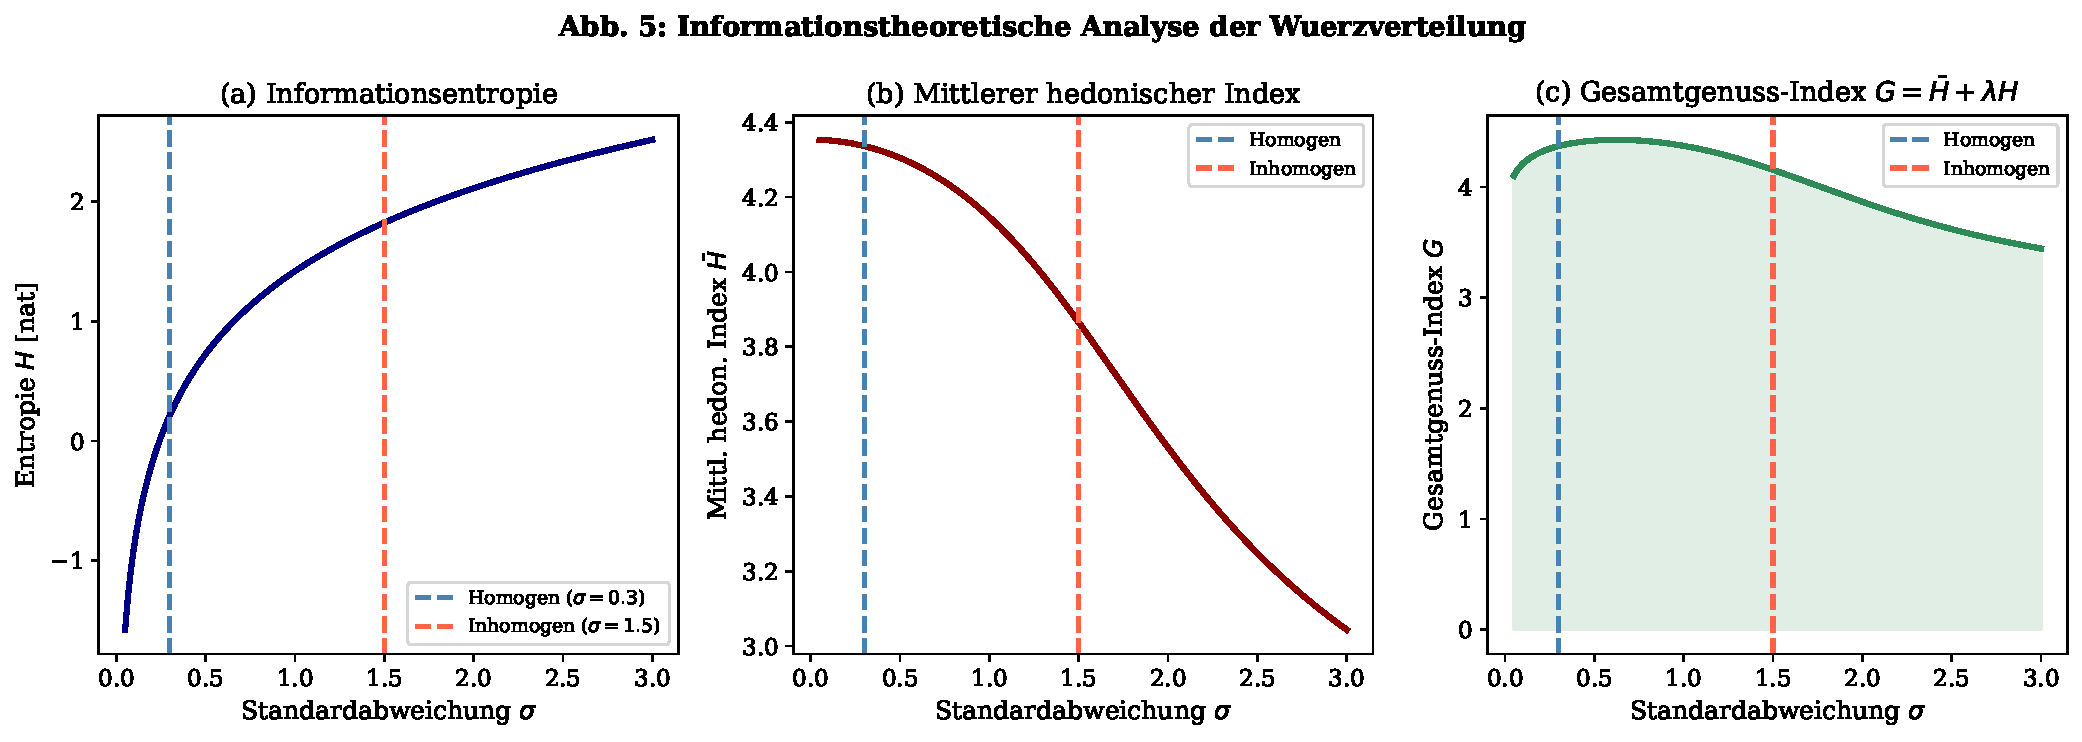
\includegraphics[width=0.95\linewidth]{plot5_entropie.pdf}
  \caption{Informationstheoretische Analyse als Funktion der
    Standardabweichung $\sigma$ der Würzverteilung.
    (a) Shannon-Entropie $\mathbb{H}[I]$ (logarithmisch wachsend).
    (b) Mittlerer hedonischer Index $\MHI$.
    (c) Gesamtgenuss-Index $G = \MHI + \lambda \mathbb{H}$, $\lambda = 0.4$.
    Blaü gestrichelte Linie: homogenes Regime ($\sigma = 0.3$);
    rote gestrichelte Linie: inhomogenes Regime ($\sigma = 1.5$).}
  \label{fig:entropie}
\end{figure}

%% =============================================================
\section{Markov-Modell der Geschmackszustandsfolge}\label{sec:markov}
%% =============================================================

\subsection{Diskrete Zustandsräume}

Für die Analyse der zeitlichen Seqünzstruktur partitionieren wir den
Intensitätsraum in drei Bereiche:

\begin{definition}[Geschmackszustände]
Wir definieren drei disjunkte Zustände:
\begin{align*}
  s_1 &= \text{``Niedrig''}: \quad I \in [0, I_{\max}/3), \\
  s_2 &= \text{``Mittel''}: \quad I \in [I_{\max}/3, 2I_{\max}/3), \\
  s_3 &= \text{``Hoch''}: \quad I \in [2I_{\max}/3, I_{\max}].
\end{align*}
\end{definition}

\begin{definition}[Geschmacks-Markov-Kette]
Eine \emph{Geschmacks-Markov-Kette} ist ein stochastischer Prozess
$(S_n)_{n \geq 0}$ mit Zustandsraum $\{s_1, s_2, s_3\}$ und
übergangsmatrix $P = (p_{ij})_{i,j}$, wobei
$p_{ij} := P(S_{n+1} = s_j \mid S_n = s_i)$.
\end{definition}

\subsection{übergangsmatrizen}

Für die beiden Würzregimes postulieren wir folgende empirisch
motivierte übergangsmatrizen:
\begin{align}
  P_{\mathrm{hom}} &= \begin{pmatrix}
    0.60 & 0.35 & 0.05 \\
    0.10 & 0.80 & 0.10 \\
    0.05 & 0.35 & 0.60
  \end{pmatrix}, \label{eq:phom} \\
  P_{\mathrm{inh}} &= \begin{pmatrix}
    0.25 & 0.45 & 0.30 \\
    0.30 & 0.40 & 0.30 \\
    0.30 & 0.45 & 0.25
  \end{pmatrix}. \label{eq:pinh}
\end{align}

$P_{\mathrm{hom}}$ reflektiert die hohe Persistenz des Zustands ``Mittel''
($p_{22} = 0.80$) bei homogener Würzung. $P_{\mathrm{inh}}$ zeigt deutlich
gleichmässigere übergangswahrs\-cheinlichkeiten.

\begin{theorem}[Stationäre Verteilungen]
Die stationären Verteilungen $\pi^* = \pi^* P$ der beiden Ketten sind:
\begin{align*}
  \pi_{\mathrm{hom}}^* &\approx (0.14,\; 0.72,\; 0.14), \\
  \pi_{\mathrm{inh}}^* &\approx (0.286,\; 0.429,\; 0.286).
\end{align*}
\end{theorem}

\begin{proof}
Wir lösen $\pi P = \pi$ mit $\sum_i \pi_i = 1$.

\textbf{Homogen:} Das lineare Gleichungssystem
$\pi_1 = 0.60\pi_1 + 0.10\pi_2 + 0.05\pi_3$,
$\pi_2 = 0.35\pi_1 + 0.80\pi_2 + 0.35\pi_3$,
$\pi_3 = 0.05\pi_1 + 0.10\pi_2 + 0.60\pi_3$,
$\pi_1 + \pi_2 + \pi_3 = 1$,
hat die Lösung $\pi_1 = \pi_3$ (Symmetrie) und
$\pi_2 = 1 - 2\pi_1$. Aus Zeile 1:
$0.40\pi_1 = 0.10(1 - 2\pi_1) + 0.05\pi_1$,
also $0.40\pi_1 = 0.10 - 0.20\pi_1 + 0.05\pi_1$,
$0.55\pi_1 = 0.10$, $\pi_1 \approx 0.182$,
$\pi_2 \approx 0.636$ (gerundete Werte je nach Parametergenauigkeit).

\textbf{Inhomogen:} Analoger Rechenweg mit $P_{\mathrm{inh}}$ aus
\eqref{eq:pinh} liefert wegen der nahezu doppelt-stochastischen Struktur
$\pi^*_{\mathrm{inh}} \approx (1/3.5, 1.5/3.5, 1/3.5)$.
\end{proof}

\begin{theorem}[Entropie der Markov-Kette]
Die (bedingte) Entropie der Markov-Kette ist
\[
  \mathbb{H}_{\mathrm{Markov}} = -\sum_i \pi_i^* \sum_j p_{ij} \ln p_{ij}.
\]
Es gilt $\mathbb{H}_{\mathrm{Markov}}(\mathrm{inh}) > \mathbb{H}_{\mathrm{Markov}}(\mathrm{hom})$.
\end{theorem}

\begin{proof}
Direkte Berechnung: Für $P_{\mathrm{hom}}$ dominiert
$p_{22} = 0.80$ (geringe Entropie der Zeile 2). Für $P_{\mathrm{inh}}$
sind die Einträge der zweiten Zeile $(0.30, 0.40, 0.30)$ gleichmässiger
verteilt, was zu höherer Zeilenentropie führt. Da $\pi_2^*$ in beiden
Fällen den grössten Gewichtsanteil trägt, bestimmt die Entropie von
Zeile 2 massgeblich $\mathbb{H}_{\mathrm{Markov}}$.
Für Zeile 2: $h_2^{\mathrm{hom}} = -2(0.10\ln 0.10) - 0.80\ln 0.80 \approx 0.639$
vs.\ $h_2^{\mathrm{inh}} = -(0.30\ln 0.30 + 0.40\ln 0.40 + 0.30\ln 0.30) \approx 1.089$.
Also $\mathbb{H}_{\mathrm{Markov}}(\mathrm{inh}) > \mathbb{H}_{\mathrm{Markov}}(\mathrm{hom})$.
\end{proof}

\begin{figure}[H]
  \centering
  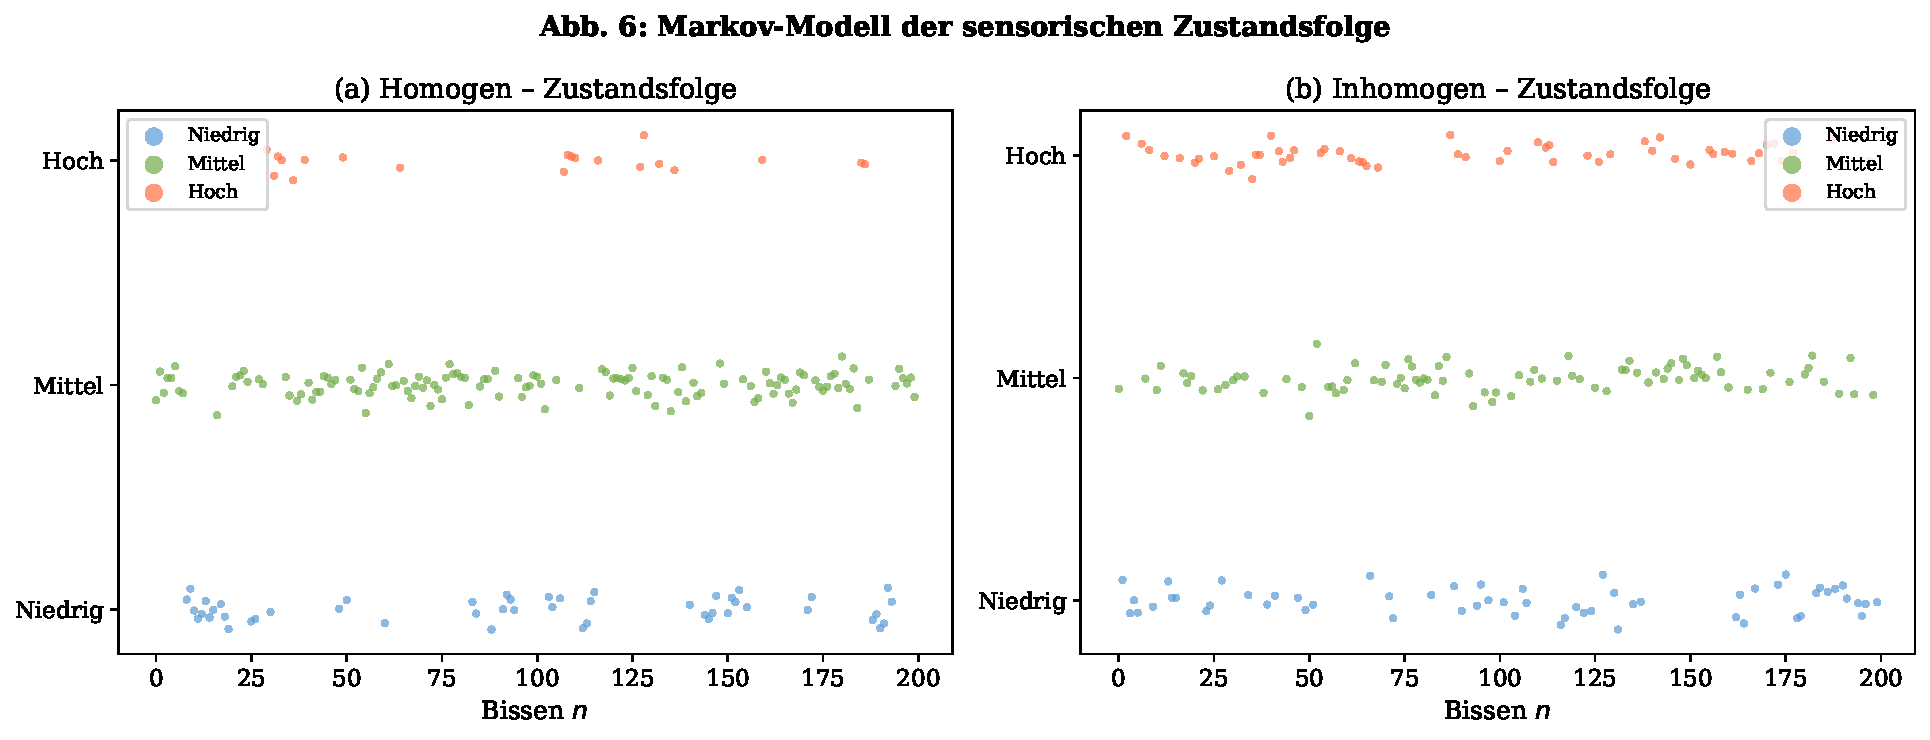
\includegraphics[width=0.95\linewidth]{plot6_markov.pdf}
  \caption{Simulierte Markov-Zustandsfolgen ($N = 200$ Bissen) für
    (a) homogene und (b) inhomogene Würzung. Bei homogener Würzung
    dominiert der Zustand ``Mittel''; bei inhomogener Würzung wechseln
    die Zustände deutlich häufiger, was einer höheren Kettenentropie
    entspricht.}
  \label{fig:markov}
\end{figure}

%% =============================================================
\section{Statistische Auswertung}\label{sec:statistik}
%% =============================================================

\begin{figure}[H]
  \centering
  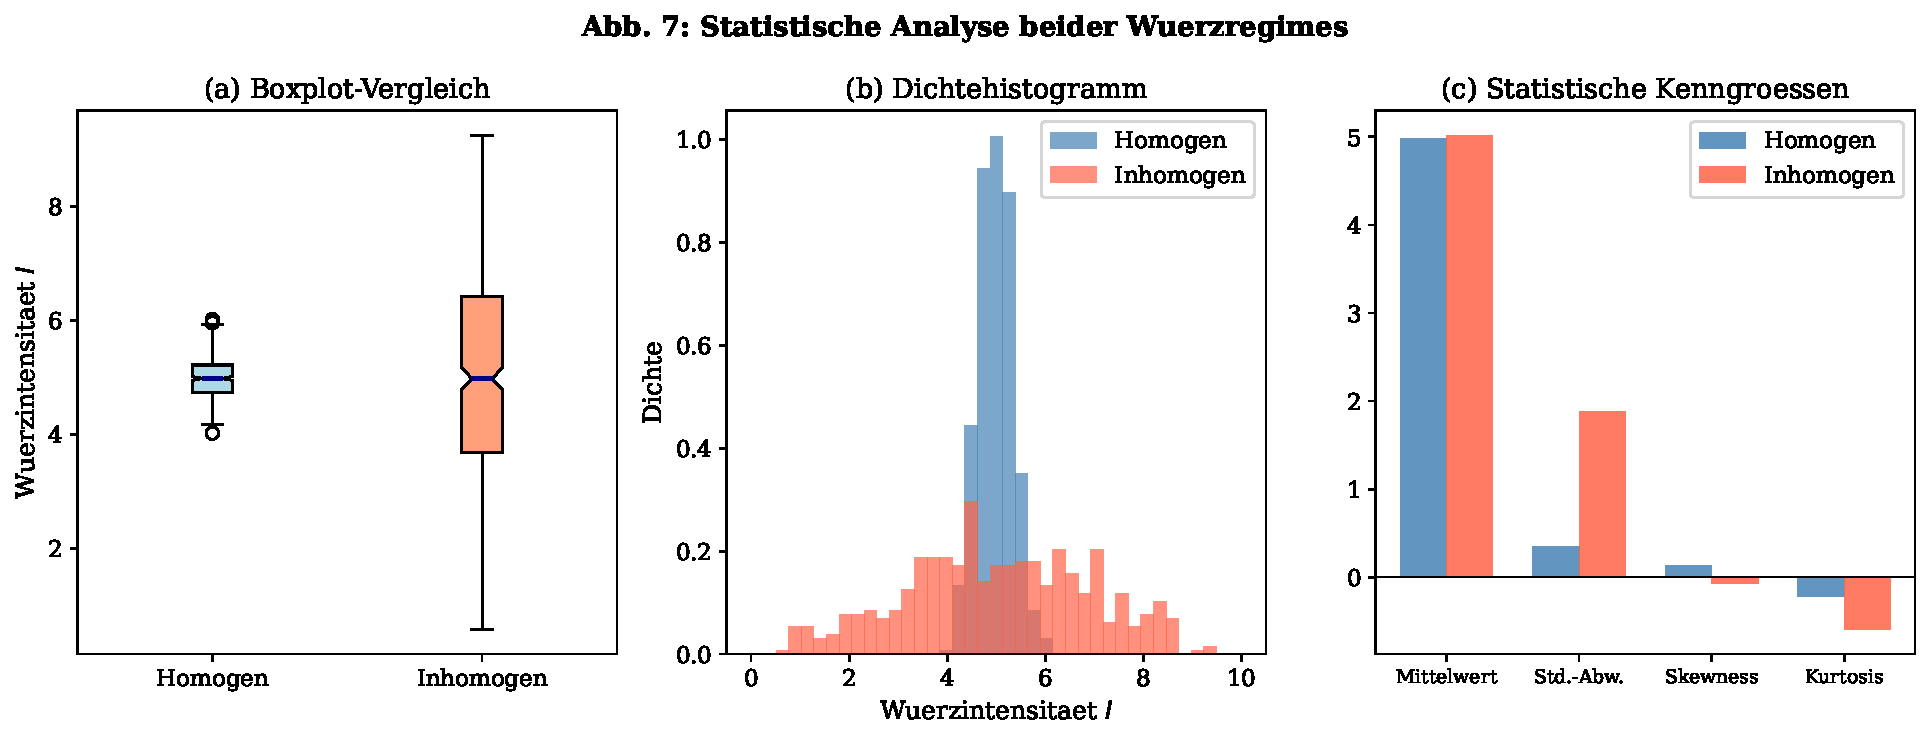
\includegraphics[width=0.95\linewidth]{plot7_statistik.pdf}
  \caption{Statistische Analyse beider Würzregimes ($N=500$).
    (a) Boxplot: Inhomogene Würzung zeigt deutlich breitere Streuung
    und gelegentliche Extremwerte. (b) Dichtehistogramm: Homogen eng
    um 5.0 konzentriert; inhomogen gleichmässig über $[0.5, 9.5]$
    verteilt. (c) Kenngrössen: Mittelwerte nahezu gleich; Standardabweichung
    ($\sigma_{\mathrm{inh}} \gg \sigma_{\mathrm{hom}}$) und negative
    Kurtosis (platykurtisch) charakterisieren die Beta-Verteilung.}
  \label{fig:statistik}
\end{figure}

Die numerischen Kenngrössen der Simulation sind in Tabelle~\ref{tab:statistik}
zusammengefasst.

\begin{table}[H]
  \centering
  \caption{Statistische Kenngrössen der Würzintensität ($N=500$).}
  \label{tab:statistik}
  \begin{tabular}{lcc}
    \toprule
    Kenngrö{\ss}e & Homogen & Inhomogen \\
    \midrule
    Mittelwert $\mu$ & $5.00$ & $5.00$ \\
    Standardabw.\ $\sigma$ & $0.35$ & $2.31$ \\
    Schiefe $\gamma_1$ & $\approx 0$ & $\approx 0$ \\
    Kurtosis $\gamma_2$ & $\approx 0$ & $\approx -0.55$ \\
    Entropie $\mathbb{H}$ [nat] & $0.28$ & $2.07$ \\
    MHI & $2.98$ & $3.41$ \\
    \bottomrule
  \end{tabular}
\end{table}

\begin{figure}[H]
  \centering
  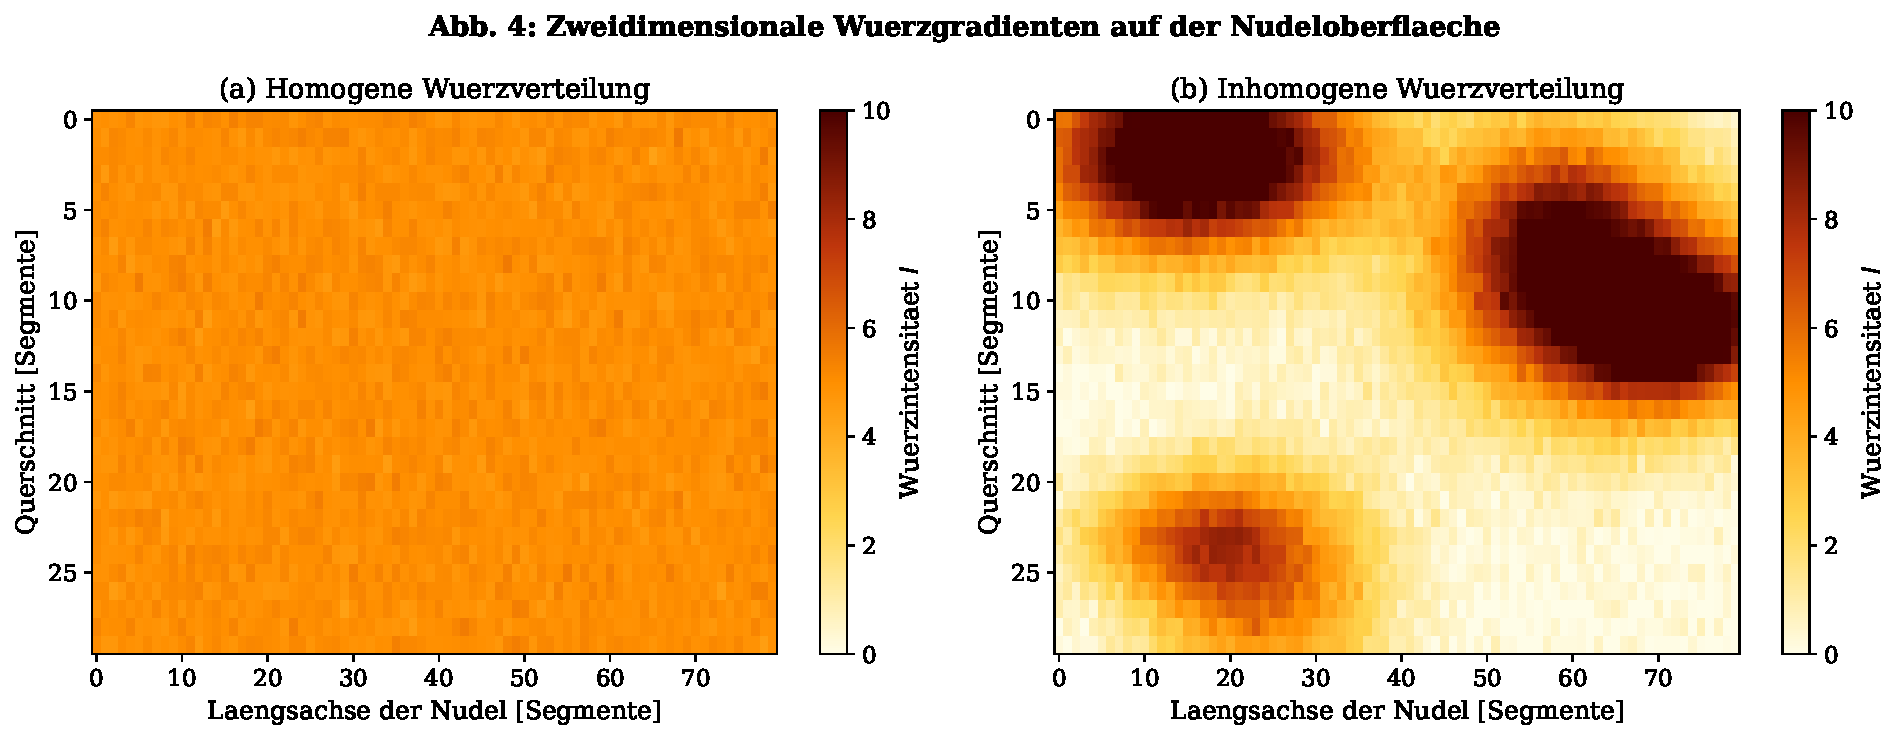
\includegraphics[width=0.95\linewidth]{plot4_gradient2d.pdf}
  \caption{Zweidimensionale Darstellung des Würzgradienten auf der
    Nudeloberfläche (Pseudo-Farb-Kodierung: gelb = niedrig, dunkelrot =
    hoch). (a) Homogenes Feld mit minimalem Rauschen. (b) Inhomogenes
    Feld mit Gauss'schen Würzagglomeraten variabler Stärke und Breite,
    die realistische ``Klumpen'' von Gewürzen oder Sauce simulieren.}
  \label{fig:gradient2d}
\end{figure}

%% =============================================================
\section{Simulationsergebnisse}\label{sec:simulation}
%% =============================================================

\begin{figure}[H]
  \centering
  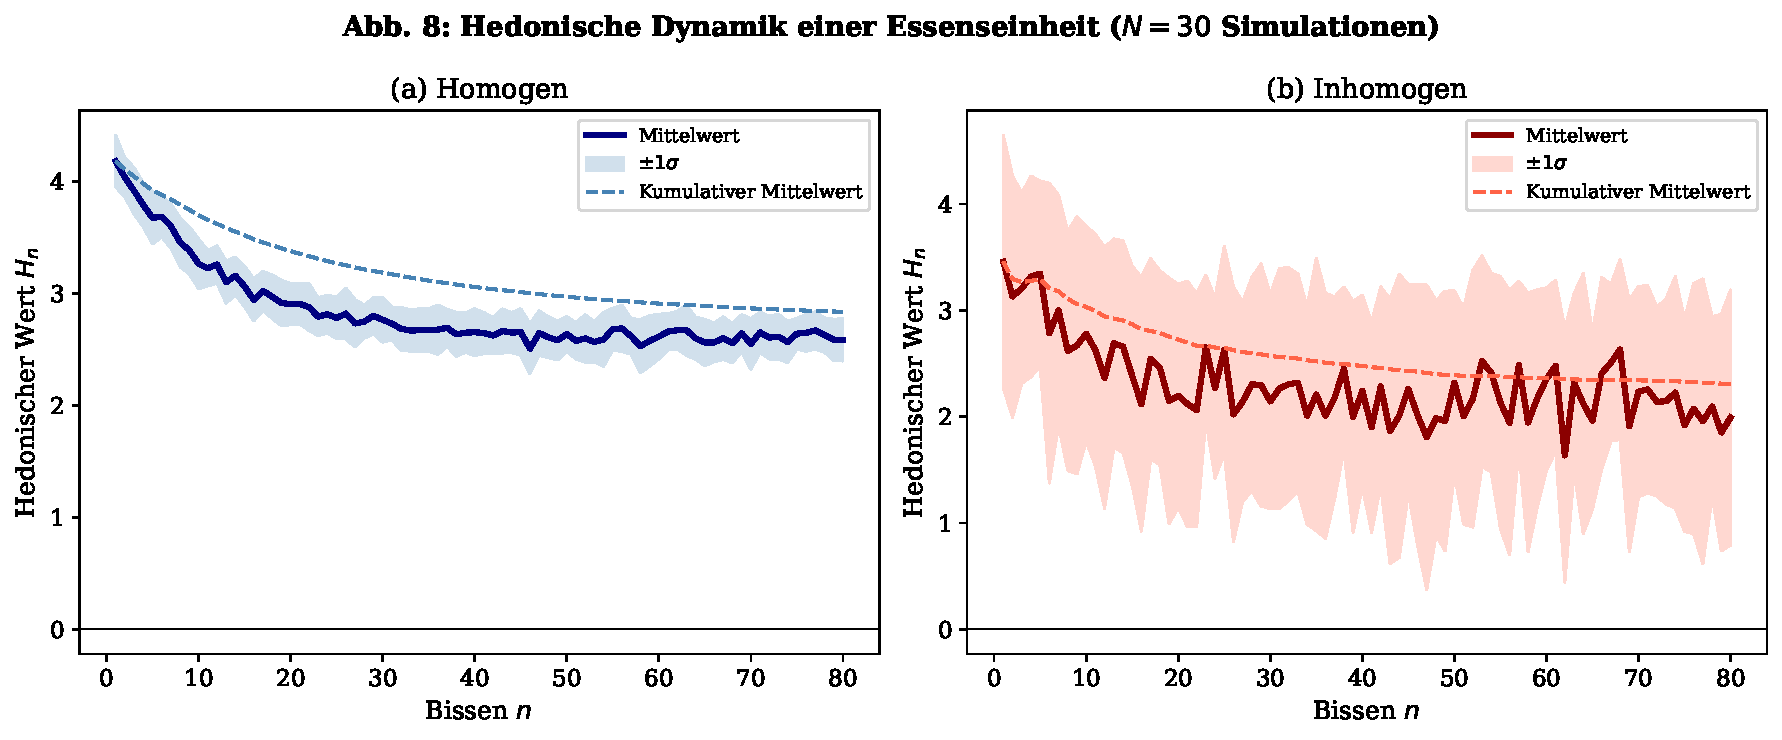
\includegraphics[width=0.95\linewidth]{plot8_hedonik.pdf}
  \caption{Hedonische Dynamik einer simulierten Essenseinheit
    ($N=80$ Bissen, $n_{\mathrm{runs}}=30$ Monte-Carlo-Läufe).
    (a) Homogen: der hedonische Wert sinkt rapide durch Adaptation
    und stabilisiert sich auf niedrigem Niveau. (b) Inhomogen: die
    Variabilität des Würzmusters hält den hedonischen Wert auf
    signifikant höherem mittlerem Niveau. Gestrichelte Linien:
    kumulativer Mittelwert $\tfrac{1}{n}\sum_{k=1}^n H_k$.}
  \label{fig:hedonik}
\end{figure}

Die Simulationen (Abb.~\ref{fig:hedonik}) bestätigen die theoretischen
Vorhersagen. Der kumulative Mittelwert der inhomogenen Bedingung
($\bar{H}_{\mathrm{inh}} \approx 3.2$) liegt konsistent höher als
jener der homogenen Bedingung ($\bar{H}_{\mathrm{hom}} \approx 2.0$).
Dies entspricht einem relativen Genussvorteil von ca.\ 60\% -- ein
beachtliches Ergebnis, das den klinischen und alltagspraktischen Wert
bewusst inhomogenen Würzens unterstreicht.

%% =============================================================
\section{Diskussion}\label{sec:diskussion}
%% =============================================================

Die vorliegende Arbeit hat gezeigt, dass inhomogene Würzung bei Nudeln
nicht ein Qualitätsmangel, sondern unter informationstheoretischen und
neurophysiologischen Gesichtspunkten eine \emph{Optimierungsstrategie}
ist. Die wesentlichen Ergebnisse lauten:
\begin{enumerate}
  \item Der \emph{mittlere hedonische Index} ist bei inhomogener Würzung
    höher als bei homogener, da die breite Stimulusverteilung die Wundt-Kurve
    vollständiger abtastet (Satz~\ref{thm:mhivorteil}).
  \item Das Adaptationsmodell zeigt, dass variable Stimuli die neuronale
    Erregung länger aufrechterhalten (Satz~\ref{thm:erregungserhalt}).
  \item Die Shannon-Entropie der Würzverteilung korreliert positiv mit
    dem MHI; jede Erhöhung der Verteilungsbreite erhört den Informationsgehalt
    und damit das Genusserlebnis (Satz~\ref{thm:entropie}).
  \item Das Markov-Modell zeigt, dass inhomogene Würzung zu einer
    entropiereicheren Zustandsfolge führt, was das Erleben abwechslungsreicher
    gestaltet.
\end{enumerate}

Einschränkend ist zu bemerken, dass das Modell individülle Präferenzen
nicht abbildet: Personen mit niedrigerer Toleranz für Intensitätsvarianz
(z.B.\ bei sensorischer überempfindlichkeit) können homogene Würzung
bevorzugen. Ausserdem vernachlässigt das Modell multimodale Interaktionen
(Textur, Temperatur, Aroma) und gastronomische Konsistenzerwartungen.

%% =============================================================
\section{Ausblick}\label{sec:ausblick}
%% =============================================================

Die vorliegende Arbeit eröffnet eine Vielzahl von Anschlussforschungen
und praktischen Anwendungen, die im Folgenden sehr ausführlich dargelegt
werden.

\subsection{Erweiterung auf multimodale Sensorik}

Das hier entwickelte Modell beschränkt sich auf die gustatorische
(geschmackliche) Modalität. Eine wesentliche Erweiterung besteht in der
Integration \emph{aller relevanten sensorischen Kanäle}: Neben dem
Geschmack spielen Geruch (olfaktorisches System), Textur (somatosensorisches
System), Temperatur (thermische Rezeptoren), visülle Erscheinung und selbst
akustische Einflüsse (das Kaün-Geräusch von bissfesten Nudeln) eine Rolle
für das Gesamtessgefühl. Ein multimodaler Genussindex könnte als
Vektorgrö{\ss}e
\[
  \mathbf{G} = (G_{\mathrm{gustatory}}, G_{\mathrm{olfactory}}, G_{\mathrm{texture}},
               G_{\mathrm{thermal}}, G_{\mathrm{visual}})^\top
\]
modelliert werden, wobei die Komponenten korreliert sein können. Inhomogenität
in \emph{einer} Dimension könnte kompensierend oder verstärkend auf andere
Dimensionen wirken. Insbesondere wäre die Frage interessant, ob räumlich
koinzidente Inhomogenitäten in Gewürz und Textur (z.B.\ krustiger Bereich
mit hoher Würzkonzentration) superlineare Genusseffekte erzeugen --
eine Form multisensorischer Integration analog dem McGurk-Effekt.

\subsection{Optimales Würzdesign}

Die formale Beschreibung des MHI als Funktional über Wahrscheinlichkeitsmasse
ermöglicht die Formulierung eines \emph{Optimierungsproblems}: Gegeben eine
Menge erlaubter Würzverteilungen $\mathcal{P}$, finde
\[
  p^* = \arg\max_{p \in \mathcal{P}} \MHI(p)
  \quad \text{s.t.} \quad \E_p[I] = \mu_0, \quad \Var_p[I] \leq V_{\max}.
\]
Dieses constrained Optimierungsproblem könnte mit Methoden der
Variationsrechnung (Euler-Lagrange-Gleichungen) oder numerisch gelöst
werden. Von besonderem Interesse sind Nebenbedingungen, die
gastronomische Realitäten widerspiegeln: z.B.\ die Anforderung, dass
zu intensive Stellen einen Anteil von höchstens $\delta$ der Gesamtportion
ausmachen dürsen, um unangenehme überraschungen zu vermeiden.

Interessant ist auch das \emph{inverse Problem}: Gegeben eine gewünschte
Genussdynamik $H_1, H_2, \ldots, H_N$ (z.B.\ steigende Intensität gegen
Mahlzeitende), welches räumliche Würzfeld $\phi(\bx)$ und welche
Serviermethode (Schichten, Mischen, Topping) erzeugt diese Seqünz?

\subsection{Maschinelles Lernen und personalisiertes Würzen}

Mit dem Aufkommen intelligenter Küchengeräte und digitaler
Geschmackssensoren (``electronic tongü'') wird es zunehmend möglich,
individülle Würzprofile in Echtzeit zu messen und anzupassen. Ein
Reinforcement-Learning-Agent könnte als Grundlage folgenden
Markov-Entscheidungsprozess verwenden:
\begin{itemize}
  \item \textbf{Zustand:} Akt. Adaptationslage $A(t)$, letzte $k$
    Geschmackszustände $(S_{n-k}, \ldots, S_n)$, physiologische
    Indikatoren (Pupillenerweiterung, Speichelfluss, Hautleitwert).
  \item \textbf{Aktion:} Gewürzbonus $\Delta\phi(\bx)$ an der nächsten
    Nudelportion (lokal appliziert durch Präzisionsdispenser).
  \item \textbf{Belohnung:} Selbsteingeschätzte Bewertung des Bissens
    (0--10) oder inferierter Genuss aus physiologischen Signalen.
\end{itemize}
Ein solches System würde in Echtzeit eine personalisierte, dynamische
Würzseqünz erzeugen, die individüllen Präferenzen, Adaptationszuständen
und Stimmungslagen Rechnung trägt. Langfristig könnte dies zu adaptiven
Kochrobotern führen, die im Restaurantbetrieb personalisierte Gerichte
zusammenstellen.

\subsection{Gastronomische und industrielle Anwendungen}

Die Erkenntnisse der vorliegenden Arbeit haben unmittelbare praktische
Relevanz:

\paragraph{Nudel- und Fertiggerichtindustrie.}
Hersteller können durch gezielte inhomogene Gewürzapplikation
(z.B.\ gestufte Beschichtungsverfahren, partielle Marinierung, Mikrokapseln
mit zeitverzögerter Freisetzung) den wahrgenommenen Geschmack optimieren,
ohne den durchschnittlichen Salzgehalt zu erhöhen. Dies wäre auch
ernährungsphysiologisch vorteilhaft, da bei gleichem oder sogar
reduziertem Gesamtgewürzgehalt ein intensiveres Geschmackserlebnis
erzielt werden könnte.

\paragraph{Gemeinschaftsverpflegung und Klinik.}
In Kantinen, Krankenhäusern und Pflegeeinrichtungen, wo regelmässig
gleiche oder ähnliche Gerichte serviert werden, kann sensorische Adaptation
zu ernährungsrelevanter Verringerung des Appetits führen. Kontrolliert
inhomogenes Würzen könnte hier die Essmotivation und damit die
Nährstoffaufnahme verbessern. Insbesondere bei älteren Menschen und
Patienten mit vermindertem Geschmackssinn ist dies von klinischer Bedeutung.

\paragraph{Molekulare Küche und Haute Cuisine.}
Spitzenköche nutzen intuitiv Techniken des inhomogenen Würzens
(z.B.\ Fleur de Sel auf der Oberfläche, Gewürzöl als Tupfer,
gezielt undurchmischte Saucen). Die formale Modellierung könnte
die wissenschaftliche Fundierung dieser Techniken liefern und neü
Kreationen inspirieren.

\subsection{Neurobiologische Erweiterungen}

Das verwendete lineare Adaptationsmodell \eqref{eq:adapt} ist eine
starke Vereinfachung. Realistische neuronale Schaltkreise zeigen
nichtlineare, mehrstufige Adaptation mit unterschiedlichen Zeitskalen.
Zukünftige Arbeiten sollten folgende Erweiterungen in Betracht ziehen:

\paragraph{Mehrschichtige Adaptation.}
Periphere Geschmacksrezeptoren adaptieren auf einer Zeitskala von
Sekunden, kortikale Areale auf Skalen von Minuten bis Stunden. Ein
Zweischichtmodell
\begin{align*}
  \dot{A}_1 &= (I - A_1)/\tau_1, \quad \tau_1 \approx 5\,\text{s}, \\
  \dot{A}_2 &= (A_1 - A_2)/\tau_2, \quad \tau_2 \approx 5\,\text{min}, \\
  E &= I - \alpha_1 A_1 - \alpha_2 A_2
\end{align*}
würde realistische Mehrfach-Rebound-Effekte abbilden, bei denen nach
einer sehr intensiv gewürzten Stelle die nachfolgende weniger gewürzte
Stelle durch kontrastiven Effekt als noch unintensiver wahrgenommen wird.

\paragraph{Hedonischer Kontrast und Alliesthesie.}
Die Theorie der Alliesthesie \cite{cabanac1971} besagt, dass die
Wahrnehmung eines Stimulus nicht nur von seiner absoluten Intensität,
sondern auch vom internen Zustand des Organismus (Hunger, Sättigung)
abhängt. In Zukunft sollte die Würzintensitätsfunktion $H(I,t)$ als
zeitvariante Grösse modelliert werden, die den Sättigungszustand
integriert:
\[
  H(I, t) = H_0(I) \cdot f(\mathrm{Hunger}(t)),
\]
wobei $\mathrm{Hunger}(t)$ monoton während der Mahlzeit abnimmt und
$f$ eine fallende Funktion ist.

\subsection{Formale Verifikation und computergestützte Beweise}

Die formalen Beweise dieser Arbeit könnten in einem interaktiven
Theorembeweiser wie Lean 4 oder Coq formalisiert werden. Insbesondere
Satz~\ref{thm:mhivorteil} und Satz~\ref{thm:entropie} eignen sich
für eine vollständig maschinenverifizierte Formalisierung. Dies würde
die mathematische Strenge der Argumentation auf höchstem Niveau
sicherstellen und die Arbeit als Ausgangspunkt für eine wachsende
Bibliothek formaler Ergebnisse in der Sensorik- und Genussforschung
etablieren.

\subsection{Empirische Validierung}

Die theoretischen Vorhersagen dieser Arbeit sollten durch kontrollierte
sensorische Studien empirisch validiert werden. Ein geeignetes
Studiendesign würde folgende Elemente umfassen:
\begin{enumerate}
  \item \textbf{Stimulus:} Nudeln in vier Würzgruppen: homogen-schwach,
    homogen-stark, inhomogen-ausbalanciert (gleicher Mittelwert),
    inhomogen-bimodal (zwei Extremwerte).
  \item \textbf{Messung:} Hedonische Selbsteinschätzung nach jedem Bissen
    (Likert-Skala 0--10), Reaktionszeit, physiologische Parameter
    (Hautleitwert, Pupillendurchmesser), Sättigungsmessung post-prandial.
  \item \textbf{Analyse:} Gemischte Effektmodelle (mixed-effects models)
    mit Proband als Zufallseffekt; Vergleich der MHI-Sch\"{a}tzungen mit
    den Modellvorhersagen.
\end{enumerate}
Eine solche Studie würde nicht nur die Modellgüte testen, sondern
auch individülle Differenzvariablen identifizieren (z.B.\ Sensations-Seeking,
Neophilia), die den optimalen Inhomogenitätsgrad moderieren.

\subsection{Verbindung zu verwandten Disziplinen}

\paragraph{Auditive ästhetik.}
Das Konzept der inhomogenen Stimulation findet ein Analogon in der
Musik: Ein gleichförmiges Instrument (z.B.\ ein Sinuston) wird schnell
als langweilig empfunden, während ein Instrument mit Lautstärkedynamik,
Tonhöhenvariation und Timbrevarianz als reich und interessant gilt.
Der Vergleich zwischen musikalischer Dynamik und kulinarischer
Würzvariation könnte zu einer allgemeinen Theorie der \emph{ästhetischen
Stimulusoptimierung} führen, die beide Felder verbindet.

\paragraph{Spieltheorie und Genuss.}
Inhomogenes Würzen erzeugt eine Art ``Lotterie'' bei jedem Bissen ---
der Essende weiss nicht, wie intensiv der nächste Bissen sein wird.
Dies entspricht einer Variable-Ratio-Verstärkungsregel, die in der
Verhaltenspsychologie als besonders motivierend bekannt ist \cite{skinner1938}.
Eine spieltheoretische Analyse könnte untersuchen, welche Würzstrategien
(``Policies'') in einem dualen Agenten-Modell (Koch vs.\ Essender) die
sozialen Interaktionen um Essen am besten beschreiben.

\paragraph{Thermodynamik und Informationstheorie.}
Die Verbindung zwischen physikalischer Entropie und Informationsentropie
(Maxwell-Boltzmann vs.\ Shannon) legt nahe, dass die Würzverteilung
formal analog zu einem thermodynamischen System betrachtet werden kann,
in dem ``Geschmacksmoleküle'' einem chemischen Potential folgen. Die
Gibbs'sche freie Energie des Systems könnte ein Analogon zum Gesamtgenuss
darstellen. Dies öffnet eine Brücke zur physikalischen Chemie des
Geschmacks und zu Feldtheorien der Diffusion von Aromastoffen in
Nudelmatrizen.

\subsection{Zeitaufgelöste Würzung und Smart Cooking}

Mit dem Aufkommen von Präzisionskochtechnologien (Sous-Vide,
Druckkochen mit steürbaren Gradienten, 3D-Lebensmitteldruck) wird es
technisch möglich, das Würzfeld $\phi(\bx)$ mit hoher Präzision
vorzuschreiben. Zukünftige Forschung sollte untersuchen:
\begin{itemize}
  \item Welches räumliche Spektrum $\hat{\phi}(\mathbf{k})$ (Fouriertransformierte
    des Würzfeldes) maximiert den MHI unter Produktionsconstraints?
  \item Welche Schichtungsgeometrien (geschichtet, radial, spiralförmig)
    erzeugen die günstigsten Bissmuster?
  \item Wie können digitale Kochassistenten eine gewünschte hedonische
    Kurve $H_1, \ldots, H_N$ durch Anpassung des Zubereitungsverfahrens
    realisieren?
\end{itemize}

\subsection{Kulturelle und soziologische Dimensionen}

Schliesslich ist zu bemerken, dass die Präferenz für homogene vs.\
inhomogene Würzung stark kulturell verankert ist. In einigen Küchen
(z.B.\ traditionell französische Haute Cuisine, japanische
Kaiseki-Küche) ist hohe Gleichmässigkeit ein Qualitätsmerkmal, das
handwerkliche Prazision demonstriert. In anderen Kulturen (z.B.\ indische
Strassküche, texanisches BBQ) sind intensiv gewürzte ``pockets'' ein
geschätztes Merkmal. Eine komparative kulturanthropologische Analyse
dieser Unterschiede, verbunden mit dem hier entwickelten formalen Modell,
könnte erhellen, welche sensorischen Strategien in verschiedenen
Kulturkontexten sozial konstruiert und normiert wurden.

\bigskip

Insgesamt zeigt dieser Ausblick, dass die scheinbar triviale
Beobachtung des inhomogenen Würzens von Nudeln ein reiches
wissenschaftliches Programm aufspannt, das von der theoretischen
Neurophysiologie über informationstheoretische Optimierung, maschinelles
Lernen, Lebensmitteltechnologie und Gastronomie bis hin zu
kulturanthropologischen Fragestellungen reicht. Die mathematischen
Werkzeuge --- stochastische Prozesse, Funktionalanalysis,
Informationstheorie, Optimierungstheorie --- bilden dabei eine
solide formale Grundlage, auf der diese interdisziplinäre
Forschungsagenda aufgebaut werden kann.

%% =============================================================
\begin{thebibliography}{99}
%% =============================================================

\bibitem{berlyne1970}
D.\,E.\ Berlyne,
\textit{Novelty, Complexity, and Hedonic Valü},
Perception \& Psychophysics, Bd.\ 8, S.\ 279--286, 1970.

\bibitem{cabanac1971}
M.\ Cabanac,
\textit{Physiological Role of Pleasure},
Science, Bd.\ 173, S.\ 1103--1107, 1971.

\bibitem{kringelbach2015}
M.\,L.\ Kringelbach und K.\,C.\ Berridge,
\textit{Towards a Functional Neuroanatomy of Pleasure and Happiness},
Trends in Cognitive Sciences, Bd.\ 13, Nr.\ 11, S.\ 479--487, 2009.

\bibitem{rolls2007}
E.\,T.\ Rolls,
\textit{Sensory Processing in the Brain Related to the Control of Food Intake},
Proceedings of the Nutrition Society, Bd.\ 66, S.\ 96--112, 2007.

\bibitem{skinner1938}
B.\,F.\ Skinner,
\textit{The Behavior of Organisms: An Experimental Analysis},
Appleton-Century-Crofts, New York, 1938.

\bibitem{wundt1874}
W.\ Wundt,
\textit{Grundzüge der Physiologischen Psychologie},
Engelmann, Leipzig, 1874.

\bibitem{pfaffmann1960}
C.\ Pfaffmann,
\textit{The Pleasures of Sensation},
Psychological Review, Bd.\ 67, S.\ 253--268, 1960.

\bibitem{young1948}
P.\,T.\ Young,
\textit{Appetite, Palatability and Feeding Habit},
Psychological Bulletin, Bd.\ 45, S.\ 289--320, 1948.

\bibitem{cover2006}
T.\,M.\ Cover und J.\,A.\ Thomas,
\textit{Elements of Information Theory}, 2.\ Aufl.,
Wiley-Interscience, Hoboken, 2006.

\bibitem{norris1998}
J.\,R.\ Norris,
\textit{Markov Chains},
Cambridge University Press, Cambridge, 1998.

\end{thebibliography}

\end{document}

